% Created by tikzDevice version 0.7.0 on 2014-07-01 17:48:08
% !TEX encoding = UTF-8 Unicode
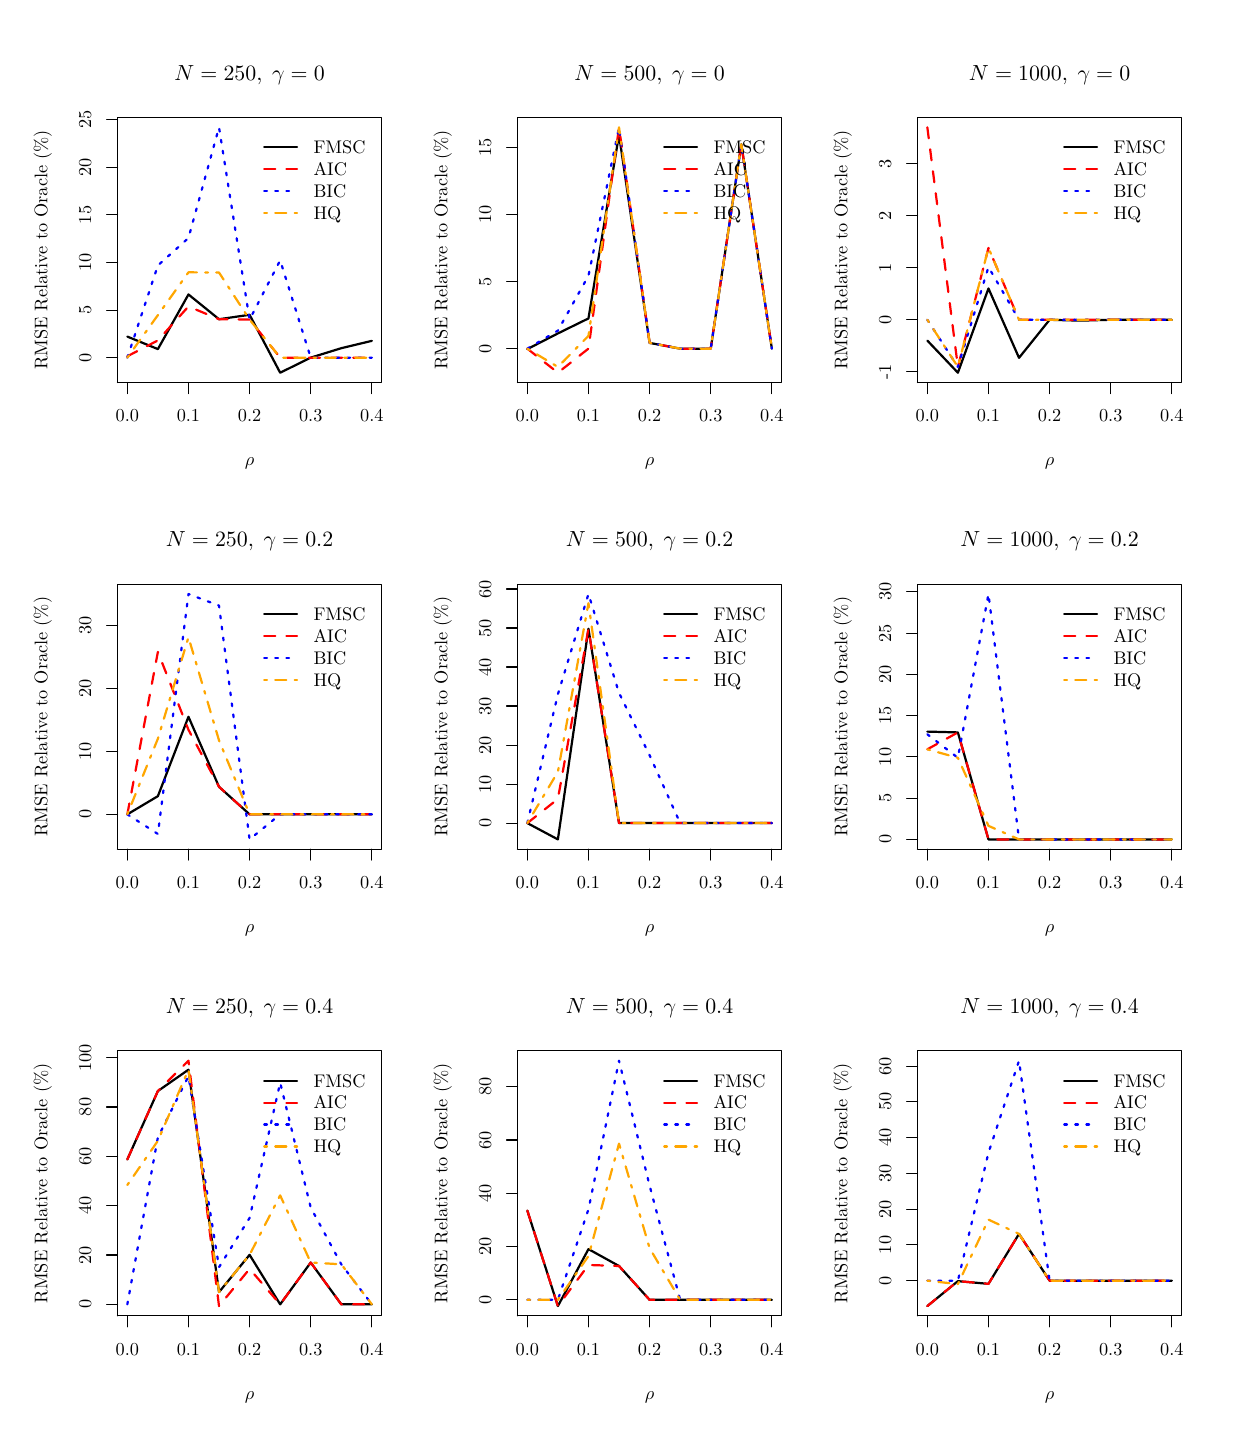
\begin{tikzpicture}[x=1pt,y=1pt]
\definecolor[named]{fillColor}{rgb}{1.00,1.00,1.00}
\path[use as bounding box,fill=fillColor,fill opacity=0.00] (0,0) rectangle (433.62,505.89);
\begin{scope}
\path[clip] ( 32.47,377.65) rectangle (127.91,473.42);
\definecolor[named]{drawColor}{rgb}{0.00,0.00,0.00}

\path[draw=drawColor,line width= 0.8pt,line join=round,line cap=round] ( 36.01,394.26) --
	( 47.05,389.74) --
	( 58.10,409.48) --
	( 69.14,400.54) --
	( 80.19,402.13) --
	( 91.24,381.20) --
	(102.28,386.65) --
	(113.33,390.07) --
	(124.37,392.72);
\end{scope}
\begin{scope}
\path[clip] (  0.00,  0.00) rectangle (433.62,505.89);
\definecolor[named]{drawColor}{rgb}{0.00,0.00,0.00}

\path[draw=drawColor,line width= 0.4pt,line join=round,line cap=round] ( 36.01,377.65) -- (124.37,377.65);

\path[draw=drawColor,line width= 0.4pt,line join=round,line cap=round] ( 36.01,377.65) -- ( 36.01,373.69);

\path[draw=drawColor,line width= 0.4pt,line join=round,line cap=round] ( 58.10,377.65) -- ( 58.10,373.69);

\path[draw=drawColor,line width= 0.4pt,line join=round,line cap=round] ( 80.19,377.65) -- ( 80.19,373.69);

\path[draw=drawColor,line width= 0.4pt,line join=round,line cap=round] (102.28,377.65) -- (102.28,373.69);

\path[draw=drawColor,line width= 0.4pt,line join=round,line cap=round] (124.37,377.65) -- (124.37,373.69);

\node[text=drawColor,anchor=base,inner sep=0pt, outer sep=0pt, scale=  0.66] at ( 36.01,363.40) {0.0};

\node[text=drawColor,anchor=base,inner sep=0pt, outer sep=0pt, scale=  0.66] at ( 58.10,363.40) {0.1};

\node[text=drawColor,anchor=base,inner sep=0pt, outer sep=0pt, scale=  0.66] at ( 80.19,363.40) {0.2};

\node[text=drawColor,anchor=base,inner sep=0pt, outer sep=0pt, scale=  0.66] at (102.28,363.40) {0.3};

\node[text=drawColor,anchor=base,inner sep=0pt, outer sep=0pt, scale=  0.66] at (124.37,363.40) {0.4};

\path[draw=drawColor,line width= 0.4pt,line join=round,line cap=round] ( 32.47,386.65) -- ( 32.47,472.62);

\path[draw=drawColor,line width= 0.4pt,line join=round,line cap=round] ( 32.47,386.65) -- ( 28.51,386.65);

\path[draw=drawColor,line width= 0.4pt,line join=round,line cap=round] ( 32.47,403.84) -- ( 28.51,403.84);

\path[draw=drawColor,line width= 0.4pt,line join=round,line cap=round] ( 32.47,421.04) -- ( 28.51,421.04);

\path[draw=drawColor,line width= 0.4pt,line join=round,line cap=round] ( 32.47,438.23) -- ( 28.51,438.23);

\path[draw=drawColor,line width= 0.4pt,line join=round,line cap=round] ( 32.47,455.43) -- ( 28.51,455.43);

\path[draw=drawColor,line width= 0.4pt,line join=round,line cap=round] ( 32.47,472.62) -- ( 28.51,472.62);

\node[text=drawColor,rotate= 90.00,anchor=base,inner sep=0pt, outer sep=0pt, scale=  0.66] at ( 22.97,386.65) {0};

\node[text=drawColor,rotate= 90.00,anchor=base,inner sep=0pt, outer sep=0pt, scale=  0.66] at ( 22.97,403.84) {5};

\node[text=drawColor,rotate= 90.00,anchor=base,inner sep=0pt, outer sep=0pt, scale=  0.66] at ( 22.97,421.04) {10};

\node[text=drawColor,rotate= 90.00,anchor=base,inner sep=0pt, outer sep=0pt, scale=  0.66] at ( 22.97,438.23) {15};

\node[text=drawColor,rotate= 90.00,anchor=base,inner sep=0pt, outer sep=0pt, scale=  0.66] at ( 22.97,455.43) {20};

\node[text=drawColor,rotate= 90.00,anchor=base,inner sep=0pt, outer sep=0pt, scale=  0.66] at ( 22.97,472.62) {25};

\path[draw=drawColor,line width= 0.4pt,line join=round,line cap=round] ( 32.47,377.65) --
	(127.91,377.65) --
	(127.91,473.42) --
	( 32.47,473.42) --
	( 32.47,377.65);
\end{scope}
\begin{scope}
\path[clip] (  0.00,337.26) rectangle (144.54,505.89);
\definecolor[named]{drawColor}{rgb}{0.00,0.00,0.00}

\node[text=drawColor,anchor=base,inner sep=0pt, outer sep=0pt, scale=  0.79] at ( 80.19,486.92) {\bfseries $N=250, \;\gamma=0$};

\node[text=drawColor,anchor=base,inner sep=0pt, outer sep=0pt, scale=  0.66] at ( 80.19,347.56) {$\rho$};

\node[text=drawColor,rotate= 90.00,anchor=base,inner sep=0pt, outer sep=0pt, scale=  0.66] at (  7.13,425.53) {RMSE Relative to Oracle (\%)};
\end{scope}
\begin{scope}
\path[clip] ( 32.47,377.65) rectangle (127.91,473.42);
\definecolor[named]{drawColor}{rgb}{1.00,0.00,0.00}

\path[draw=drawColor,line width= 0.8pt,dash pattern=on 4pt off 4pt ,line join=round,line cap=round] ( 36.01,387.14) --
	( 47.05,392.87) --
	( 58.10,405.15) --
	( 69.14,400.54) --
	( 80.19,400.39) --
	( 91.24,386.65) --
	(102.28,386.65) --
	(113.33,386.65) --
	(124.37,386.65);
\definecolor[named]{drawColor}{rgb}{0.00,0.00,1.00}

\path[draw=drawColor,line width= 0.8pt,dash pattern=on 1pt off 3pt ,line join=round,line cap=round] ( 36.01,386.65) --
	( 47.05,419.96) --
	( 58.10,429.89) --
	( 69.14,469.87) --
	( 80.19,400.39) --
	( 91.24,421.81) --
	(102.28,386.65) --
	(113.33,386.65) --
	(124.37,386.65);
\definecolor[named]{drawColor}{rgb}{1.00,0.65,0.00}

\path[draw=drawColor,line width= 0.8pt,dash pattern=on 1pt off 3pt on 4pt off 3pt ,line join=round,line cap=round] ( 36.01,386.65) --
	( 47.05,402.01) --
	( 58.10,417.48) --
	( 69.14,417.41) --
	( 80.19,400.39) --
	( 91.24,386.65) --
	(102.28,386.65) --
	(113.33,386.65) --
	(124.37,386.65);
\definecolor[named]{drawColor}{rgb}{0.00,0.00,0.00}

\path[draw=drawColor,line width= 0.8pt,line join=round,line cap=round] ( 85.47,462.63) -- ( 97.35,462.63);
\definecolor[named]{drawColor}{rgb}{1.00,0.00,0.00}

\path[draw=drawColor,line width= 0.8pt,dash pattern=on 4pt off 4pt ,line join=round,line cap=round] ( 85.47,454.71) -- ( 97.35,454.71);
\definecolor[named]{drawColor}{rgb}{0.00,0.00,1.00}

\path[draw=drawColor,line width= 0.8pt,dash pattern=on 1pt off 3pt ,line join=round,line cap=round] ( 85.47,446.79) -- ( 97.35,446.79);
\definecolor[named]{drawColor}{rgb}{1.00,0.65,0.00}

\path[draw=drawColor,line width= 0.8pt,dash pattern=on 1pt off 3pt on 4pt off 3pt ,line join=round,line cap=round] ( 85.47,438.87) -- ( 97.35,438.87);
\definecolor[named]{drawColor}{rgb}{0.00,0.00,0.00}

\node[text=drawColor,anchor=base west,inner sep=0pt, outer sep=0pt, scale=  0.66] at (103.29,460.35) {FMSC};

\node[text=drawColor,anchor=base west,inner sep=0pt, outer sep=0pt, scale=  0.66] at (103.29,452.43) {AIC};

\node[text=drawColor,anchor=base west,inner sep=0pt, outer sep=0pt, scale=  0.66] at (103.29,444.51) {BIC};

\node[text=drawColor,anchor=base west,inner sep=0pt, outer sep=0pt, scale=  0.66] at (103.29,436.59) {HQ};
\end{scope}
\begin{scope}
\path[clip] (177.01,377.65) rectangle (272.45,473.42);
\definecolor[named]{drawColor}{rgb}{0.00,0.00,0.00}

\path[draw=drawColor,line width= 0.8pt,line join=round,line cap=round] (180.55,389.74) --
	(191.59,395.40) --
	(202.64,400.82) --
	(213.68,467.22) --
	(224.73,391.98) --
	(235.78,389.90) --
	(246.82,389.90) --
	(257.87,463.76) --
	(268.91,389.90);
\end{scope}
\begin{scope}
\path[clip] (  0.00,  0.00) rectangle (433.62,505.89);
\definecolor[named]{drawColor}{rgb}{0.00,0.00,0.00}

\path[draw=drawColor,line width= 0.4pt,line join=round,line cap=round] (180.55,377.65) -- (268.91,377.65);

\path[draw=drawColor,line width= 0.4pt,line join=round,line cap=round] (180.55,377.65) -- (180.55,373.69);

\path[draw=drawColor,line width= 0.4pt,line join=round,line cap=round] (202.64,377.65) -- (202.64,373.69);

\path[draw=drawColor,line width= 0.4pt,line join=round,line cap=round] (224.73,377.65) -- (224.73,373.69);

\path[draw=drawColor,line width= 0.4pt,line join=round,line cap=round] (246.82,377.65) -- (246.82,373.69);

\path[draw=drawColor,line width= 0.4pt,line join=round,line cap=round] (268.91,377.65) -- (268.91,373.69);

\node[text=drawColor,anchor=base,inner sep=0pt, outer sep=0pt, scale=  0.66] at (180.55,363.40) {0.0};

\node[text=drawColor,anchor=base,inner sep=0pt, outer sep=0pt, scale=  0.66] at (202.64,363.40) {0.1};

\node[text=drawColor,anchor=base,inner sep=0pt, outer sep=0pt, scale=  0.66] at (224.73,363.40) {0.2};

\node[text=drawColor,anchor=base,inner sep=0pt, outer sep=0pt, scale=  0.66] at (246.82,363.40) {0.3};

\node[text=drawColor,anchor=base,inner sep=0pt, outer sep=0pt, scale=  0.66] at (268.91,363.40) {0.4};

\path[draw=drawColor,line width= 0.4pt,line join=round,line cap=round] (177.01,389.90) -- (177.01,462.72);

\path[draw=drawColor,line width= 0.4pt,line join=round,line cap=round] (177.01,389.90) -- (173.05,389.90);

\path[draw=drawColor,line width= 0.4pt,line join=round,line cap=round] (177.01,414.17) -- (173.05,414.17);

\path[draw=drawColor,line width= 0.4pt,line join=round,line cap=round] (177.01,438.45) -- (173.05,438.45);

\path[draw=drawColor,line width= 0.4pt,line join=round,line cap=round] (177.01,462.72) -- (173.05,462.72);

\node[text=drawColor,rotate= 90.00,anchor=base,inner sep=0pt, outer sep=0pt, scale=  0.66] at (167.51,389.90) {0};

\node[text=drawColor,rotate= 90.00,anchor=base,inner sep=0pt, outer sep=0pt, scale=  0.66] at (167.51,414.17) {5};

\node[text=drawColor,rotate= 90.00,anchor=base,inner sep=0pt, outer sep=0pt, scale=  0.66] at (167.51,438.45) {10};

\node[text=drawColor,rotate= 90.00,anchor=base,inner sep=0pt, outer sep=0pt, scale=  0.66] at (167.51,462.72) {15};

\path[draw=drawColor,line width= 0.4pt,line join=round,line cap=round] (177.01,377.65) --
	(272.45,377.65) --
	(272.45,473.42) --
	(177.01,473.42) --
	(177.01,377.65);
\end{scope}
\begin{scope}
\path[clip] (144.54,337.26) rectangle (289.08,505.89);
\definecolor[named]{drawColor}{rgb}{0.00,0.00,0.00}

\node[text=drawColor,anchor=base,inner sep=0pt, outer sep=0pt, scale=  0.79] at (224.73,486.92) {\bfseries $N=500, \;\gamma=0$};

\node[text=drawColor,anchor=base,inner sep=0pt, outer sep=0pt, scale=  0.66] at (224.73,347.56) {$\rho$};

\node[text=drawColor,rotate= 90.00,anchor=base,inner sep=0pt, outer sep=0pt, scale=  0.66] at (151.67,425.53) {RMSE Relative to Oracle (\%)};
\end{scope}
\begin{scope}
\path[clip] (177.01,377.65) rectangle (272.45,473.42);
\definecolor[named]{drawColor}{rgb}{1.00,0.00,0.00}

\path[draw=drawColor,line width= 0.8pt,dash pattern=on 4pt off 4pt ,line join=round,line cap=round] (180.55,389.90) --
	(191.59,381.20) --
	(202.64,389.91) --
	(213.68,469.87) --
	(224.73,392.02) --
	(235.78,389.90) --
	(246.82,389.90) --
	(257.87,463.76) --
	(268.91,389.90);
\definecolor[named]{drawColor}{rgb}{0.00,0.00,1.00}

\path[draw=drawColor,line width= 0.8pt,dash pattern=on 1pt off 3pt ,line join=round,line cap=round] (180.55,389.90) --
	(191.59,396.41) --
	(202.64,416.25) --
	(213.68,469.87) --
	(224.73,392.02) --
	(235.78,389.90) --
	(246.82,389.90) --
	(257.87,463.76) --
	(268.91,389.90);
\definecolor[named]{drawColor}{rgb}{1.00,0.65,0.00}

\path[draw=drawColor,line width= 0.8pt,dash pattern=on 1pt off 3pt on 4pt off 3pt ,line join=round,line cap=round] (180.55,389.90) --
	(191.59,383.30) --
	(202.64,394.53) --
	(213.68,469.87) --
	(224.73,392.02) --
	(235.78,389.90) --
	(246.82,389.90) --
	(257.87,463.76) --
	(268.91,389.90);
\definecolor[named]{drawColor}{rgb}{0.00,0.00,0.00}

\path[draw=drawColor,line width= 0.8pt,line join=round,line cap=round] (230.01,462.63) -- (241.89,462.63);
\definecolor[named]{drawColor}{rgb}{1.00,0.00,0.00}

\path[draw=drawColor,line width= 0.8pt,dash pattern=on 4pt off 4pt ,line join=round,line cap=round] (230.01,454.71) -- (241.89,454.71);
\definecolor[named]{drawColor}{rgb}{0.00,0.00,1.00}

\path[draw=drawColor,line width= 0.8pt,dash pattern=on 1pt off 3pt ,line join=round,line cap=round] (230.01,446.79) -- (241.89,446.79);
\definecolor[named]{drawColor}{rgb}{1.00,0.65,0.00}

\path[draw=drawColor,line width= 0.8pt,dash pattern=on 1pt off 3pt on 4pt off 3pt ,line join=round,line cap=round] (230.01,438.87) -- (241.89,438.87);
\definecolor[named]{drawColor}{rgb}{0.00,0.00,0.00}

\node[text=drawColor,anchor=base west,inner sep=0pt, outer sep=0pt, scale=  0.66] at (247.83,460.35) {FMSC};

\node[text=drawColor,anchor=base west,inner sep=0pt, outer sep=0pt, scale=  0.66] at (247.83,452.43) {AIC};

\node[text=drawColor,anchor=base west,inner sep=0pt, outer sep=0pt, scale=  0.66] at (247.83,444.51) {BIC};

\node[text=drawColor,anchor=base west,inner sep=0pt, outer sep=0pt, scale=  0.66] at (247.83,436.59) {HQ};
\end{scope}
\begin{scope}
\path[clip] (321.55,377.65) rectangle (416.99,473.42);
\definecolor[named]{drawColor}{rgb}{0.00,0.00,0.00}

\path[draw=drawColor,line width= 0.8pt,line join=round,line cap=round] (325.09,392.82) --
	(336.13,381.20) --
	(347.18,411.65) --
	(358.22,386.58) --
	(369.27,400.33) --
	(380.32,400.02) --
	(391.36,400.33) --
	(402.41,400.33) --
	(413.45,400.33);
\end{scope}
\begin{scope}
\path[clip] (  0.00,  0.00) rectangle (433.62,505.89);
\definecolor[named]{drawColor}{rgb}{0.00,0.00,0.00}

\path[draw=drawColor,line width= 0.4pt,line join=round,line cap=round] (325.09,377.65) -- (413.45,377.65);

\path[draw=drawColor,line width= 0.4pt,line join=round,line cap=round] (325.09,377.65) -- (325.09,373.69);

\path[draw=drawColor,line width= 0.4pt,line join=round,line cap=round] (347.18,377.65) -- (347.18,373.69);

\path[draw=drawColor,line width= 0.4pt,line join=round,line cap=round] (369.27,377.65) -- (369.27,373.69);

\path[draw=drawColor,line width= 0.4pt,line join=round,line cap=round] (391.36,377.65) -- (391.36,373.69);

\path[draw=drawColor,line width= 0.4pt,line join=round,line cap=round] (413.45,377.65) -- (413.45,373.69);

\node[text=drawColor,anchor=base,inner sep=0pt, outer sep=0pt, scale=  0.66] at (325.09,363.40) {0.0};

\node[text=drawColor,anchor=base,inner sep=0pt, outer sep=0pt, scale=  0.66] at (347.18,363.40) {0.1};

\node[text=drawColor,anchor=base,inner sep=0pt, outer sep=0pt, scale=  0.66] at (369.27,363.40) {0.2};

\node[text=drawColor,anchor=base,inner sep=0pt, outer sep=0pt, scale=  0.66] at (391.36,363.40) {0.3};

\node[text=drawColor,anchor=base,inner sep=0pt, outer sep=0pt, scale=  0.66] at (413.45,363.40) {0.4};

\path[draw=drawColor,line width= 0.4pt,line join=round,line cap=round] (321.55,381.55) -- (321.55,456.69);

\path[draw=drawColor,line width= 0.4pt,line join=round,line cap=round] (321.55,381.55) -- (317.59,381.55);

\path[draw=drawColor,line width= 0.4pt,line join=round,line cap=round] (321.55,400.33) -- (317.59,400.33);

\path[draw=drawColor,line width= 0.4pt,line join=round,line cap=round] (321.55,419.12) -- (317.59,419.12);

\path[draw=drawColor,line width= 0.4pt,line join=round,line cap=round] (321.55,437.91) -- (317.59,437.91);

\path[draw=drawColor,line width= 0.4pt,line join=round,line cap=round] (321.55,456.69) -- (317.59,456.69);

\node[text=drawColor,rotate= 90.00,anchor=base,inner sep=0pt, outer sep=0pt, scale=  0.66] at (312.05,381.55) {-1};

\node[text=drawColor,rotate= 90.00,anchor=base,inner sep=0pt, outer sep=0pt, scale=  0.66] at (312.05,400.33) {0};

\node[text=drawColor,rotate= 90.00,anchor=base,inner sep=0pt, outer sep=0pt, scale=  0.66] at (312.05,419.12) {1};

\node[text=drawColor,rotate= 90.00,anchor=base,inner sep=0pt, outer sep=0pt, scale=  0.66] at (312.05,437.91) {2};

\node[text=drawColor,rotate= 90.00,anchor=base,inner sep=0pt, outer sep=0pt, scale=  0.66] at (312.05,456.69) {3};

\path[draw=drawColor,line width= 0.4pt,line join=round,line cap=round] (321.55,377.65) --
	(416.99,377.65) --
	(416.99,473.42) --
	(321.55,473.42) --
	(321.55,377.65);
\end{scope}
\begin{scope}
\path[clip] (289.08,337.26) rectangle (433.62,505.89);
\definecolor[named]{drawColor}{rgb}{0.00,0.00,0.00}

\node[text=drawColor,anchor=base,inner sep=0pt, outer sep=0pt, scale=  0.79] at (369.27,486.92) {\bfseries $N=1000, \;\gamma=0$};

\node[text=drawColor,anchor=base,inner sep=0pt, outer sep=0pt, scale=  0.66] at (369.27,347.56) {$\rho$};

\node[text=drawColor,rotate= 90.00,anchor=base,inner sep=0pt, outer sep=0pt, scale=  0.66] at (296.21,425.53) {RMSE Relative to Oracle (\%)};
\end{scope}
\begin{scope}
\path[clip] (321.55,377.65) rectangle (416.99,473.42);
\definecolor[named]{drawColor}{rgb}{1.00,0.00,0.00}

\path[draw=drawColor,line width= 0.8pt,dash pattern=on 4pt off 4pt ,line join=round,line cap=round] (325.09,469.87) --
	(336.13,383.29) --
	(347.18,426.30) --
	(358.22,400.33) --
	(369.27,400.33) --
	(380.32,400.33) --
	(391.36,400.33) --
	(402.41,400.33) --
	(413.45,400.33);
\definecolor[named]{drawColor}{rgb}{0.00,0.00,1.00}

\path[draw=drawColor,line width= 0.8pt,dash pattern=on 1pt off 3pt ,line join=round,line cap=round] (325.09,400.33) --
	(336.13,383.29) --
	(347.18,419.40) --
	(358.22,400.33) --
	(369.27,400.33) --
	(380.32,400.33) --
	(391.36,400.33) --
	(402.41,400.33) --
	(413.45,400.33);
\definecolor[named]{drawColor}{rgb}{1.00,0.65,0.00}

\path[draw=drawColor,line width= 0.8pt,dash pattern=on 1pt off 3pt on 4pt off 3pt ,line join=round,line cap=round] (325.09,400.33) --
	(336.13,383.29) --
	(347.18,426.30) --
	(358.22,400.33) --
	(369.27,400.33) --
	(380.32,400.33) --
	(391.36,400.33) --
	(402.41,400.33) --
	(413.45,400.33);
\definecolor[named]{drawColor}{rgb}{0.00,0.00,0.00}

\path[draw=drawColor,line width= 0.8pt,line join=round,line cap=round] (374.55,462.63) -- (386.43,462.63);
\definecolor[named]{drawColor}{rgb}{1.00,0.00,0.00}

\path[draw=drawColor,line width= 0.8pt,dash pattern=on 4pt off 4pt ,line join=round,line cap=round] (374.55,454.71) -- (386.43,454.71);
\definecolor[named]{drawColor}{rgb}{0.00,0.00,1.00}

\path[draw=drawColor,line width= 0.8pt,dash pattern=on 1pt off 3pt ,line join=round,line cap=round] (374.55,446.79) -- (386.43,446.79);
\definecolor[named]{drawColor}{rgb}{1.00,0.65,0.00}

\path[draw=drawColor,line width= 0.8pt,dash pattern=on 1pt off 3pt on 4pt off 3pt ,line join=round,line cap=round] (374.55,438.87) -- (386.43,438.87);
\definecolor[named]{drawColor}{rgb}{0.00,0.00,0.00}

\node[text=drawColor,anchor=base west,inner sep=0pt, outer sep=0pt, scale=  0.66] at (392.37,460.35) {FMSC};

\node[text=drawColor,anchor=base west,inner sep=0pt, outer sep=0pt, scale=  0.66] at (392.37,452.43) {AIC};

\node[text=drawColor,anchor=base west,inner sep=0pt, outer sep=0pt, scale=  0.66] at (392.37,444.51) {BIC};

\node[text=drawColor,anchor=base west,inner sep=0pt, outer sep=0pt, scale=  0.66] at (392.37,436.59) {HQ};
\end{scope}
\begin{scope}
\path[clip] ( 32.47,209.02) rectangle (127.91,304.79);
\definecolor[named]{drawColor}{rgb}{0.00,0.00,0.00}

\path[draw=drawColor,line width= 0.8pt,line join=round,line cap=round] ( 36.01,221.62) --
	( 47.05,228.19) --
	( 58.10,256.88) --
	( 69.14,231.58) --
	( 80.19,221.62) --
	( 91.24,221.62) --
	(102.28,221.62) --
	(113.33,221.62) --
	(124.37,221.62);
\end{scope}
\begin{scope}
\path[clip] (  0.00,  0.00) rectangle (433.62,505.89);
\definecolor[named]{drawColor}{rgb}{0.00,0.00,0.00}

\path[draw=drawColor,line width= 0.4pt,line join=round,line cap=round] ( 36.01,209.02) -- (124.37,209.02);

\path[draw=drawColor,line width= 0.4pt,line join=round,line cap=round] ( 36.01,209.02) -- ( 36.01,205.06);

\path[draw=drawColor,line width= 0.4pt,line join=round,line cap=round] ( 58.10,209.02) -- ( 58.10,205.06);

\path[draw=drawColor,line width= 0.4pt,line join=round,line cap=round] ( 80.19,209.02) -- ( 80.19,205.06);

\path[draw=drawColor,line width= 0.4pt,line join=round,line cap=round] (102.28,209.02) -- (102.28,205.06);

\path[draw=drawColor,line width= 0.4pt,line join=round,line cap=round] (124.37,209.02) -- (124.37,205.06);

\node[text=drawColor,anchor=base,inner sep=0pt, outer sep=0pt, scale=  0.66] at ( 36.01,194.77) {0.0};

\node[text=drawColor,anchor=base,inner sep=0pt, outer sep=0pt, scale=  0.66] at ( 58.10,194.77) {0.1};

\node[text=drawColor,anchor=base,inner sep=0pt, outer sep=0pt, scale=  0.66] at ( 80.19,194.77) {0.2};

\node[text=drawColor,anchor=base,inner sep=0pt, outer sep=0pt, scale=  0.66] at (102.28,194.77) {0.3};

\node[text=drawColor,anchor=base,inner sep=0pt, outer sep=0pt, scale=  0.66] at (124.37,194.77) {0.4};

\path[draw=drawColor,line width= 0.4pt,line join=round,line cap=round] ( 32.47,221.62) -- ( 32.47,290.00);

\path[draw=drawColor,line width= 0.4pt,line join=round,line cap=round] ( 32.47,221.62) -- ( 28.51,221.62);

\path[draw=drawColor,line width= 0.4pt,line join=round,line cap=round] ( 32.47,244.41) -- ( 28.51,244.41);

\path[draw=drawColor,line width= 0.4pt,line join=round,line cap=round] ( 32.47,267.20) -- ( 28.51,267.20);

\path[draw=drawColor,line width= 0.4pt,line join=round,line cap=round] ( 32.47,290.00) -- ( 28.51,290.00);

\node[text=drawColor,rotate= 90.00,anchor=base,inner sep=0pt, outer sep=0pt, scale=  0.66] at ( 22.97,221.62) {0};

\node[text=drawColor,rotate= 90.00,anchor=base,inner sep=0pt, outer sep=0pt, scale=  0.66] at ( 22.97,244.41) {10};

\node[text=drawColor,rotate= 90.00,anchor=base,inner sep=0pt, outer sep=0pt, scale=  0.66] at ( 22.97,267.20) {20};

\node[text=drawColor,rotate= 90.00,anchor=base,inner sep=0pt, outer sep=0pt, scale=  0.66] at ( 22.97,290.00) {30};

\path[draw=drawColor,line width= 0.4pt,line join=round,line cap=round] ( 32.47,209.02) --
	(127.91,209.02) --
	(127.91,304.79) --
	( 32.47,304.79) --
	( 32.47,209.02);
\end{scope}
\begin{scope}
\path[clip] (  0.00,168.63) rectangle (144.54,337.26);
\definecolor[named]{drawColor}{rgb}{0.00,0.00,0.00}

\node[text=drawColor,anchor=base,inner sep=0pt, outer sep=0pt, scale=  0.79] at ( 80.19,318.29) {\bfseries $N=250, \;\gamma=0.2$};

\node[text=drawColor,anchor=base,inner sep=0pt, outer sep=0pt, scale=  0.66] at ( 80.19,178.93) {$\rho$};

\node[text=drawColor,rotate= 90.00,anchor=base,inner sep=0pt, outer sep=0pt, scale=  0.66] at (  7.13,256.90) {RMSE Relative to Oracle (\%)};
\end{scope}
\begin{scope}
\path[clip] ( 32.47,209.02) rectangle (127.91,304.79);
\definecolor[named]{drawColor}{rgb}{1.00,0.00,0.00}

\path[draw=drawColor,line width= 0.8pt,dash pattern=on 4pt off 4pt ,line join=round,line cap=round] ( 36.01,221.62) --
	( 47.05,280.31) --
	( 58.10,252.18) --
	( 69.14,231.58) --
	( 80.19,221.62) --
	( 91.24,221.62) --
	(102.28,221.62) --
	(113.33,221.62) --
	(124.37,221.62);
\definecolor[named]{drawColor}{rgb}{0.00,0.00,1.00}

\path[draw=drawColor,line width= 0.8pt,dash pattern=on 1pt off 3pt ,line join=round,line cap=round] ( 36.01,221.62) --
	( 47.05,214.53) --
	( 58.10,301.24) --
	( 69.14,297.05) --
	( 80.19,212.57) --
	( 91.24,221.62) --
	(102.28,221.62) --
	(113.33,221.62) --
	(124.37,221.62);
\definecolor[named]{drawColor}{rgb}{1.00,0.65,0.00}

\path[draw=drawColor,line width= 0.8pt,dash pattern=on 1pt off 3pt on 4pt off 3pt ,line join=round,line cap=round] ( 36.01,221.62) --
	( 47.05,248.96) --
	( 58.10,285.60) --
	( 69.14,248.35) --
	( 80.19,221.62) --
	( 91.24,221.62) --
	(102.28,221.62) --
	(113.33,221.62) --
	(124.37,221.62);
\definecolor[named]{drawColor}{rgb}{0.00,0.00,0.00}

\path[draw=drawColor,line width= 0.8pt,line join=round,line cap=round] ( 85.47,294.00) -- ( 97.35,294.00);
\definecolor[named]{drawColor}{rgb}{1.00,0.00,0.00}

\path[draw=drawColor,line width= 0.8pt,dash pattern=on 4pt off 4pt ,line join=round,line cap=round] ( 85.47,286.08) -- ( 97.35,286.08);
\definecolor[named]{drawColor}{rgb}{0.00,0.00,1.00}

\path[draw=drawColor,line width= 0.8pt,dash pattern=on 1pt off 3pt ,line join=round,line cap=round] ( 85.47,278.16) -- ( 97.35,278.16);
\definecolor[named]{drawColor}{rgb}{1.00,0.65,0.00}

\path[draw=drawColor,line width= 0.8pt,dash pattern=on 1pt off 3pt on 4pt off 3pt ,line join=round,line cap=round] ( 85.47,270.24) -- ( 97.35,270.24);
\definecolor[named]{drawColor}{rgb}{0.00,0.00,0.00}

\node[text=drawColor,anchor=base west,inner sep=0pt, outer sep=0pt, scale=  0.66] at (103.29,291.72) {FMSC};

\node[text=drawColor,anchor=base west,inner sep=0pt, outer sep=0pt, scale=  0.66] at (103.29,283.80) {AIC};

\node[text=drawColor,anchor=base west,inner sep=0pt, outer sep=0pt, scale=  0.66] at (103.29,275.88) {BIC};

\node[text=drawColor,anchor=base west,inner sep=0pt, outer sep=0pt, scale=  0.66] at (103.29,267.96) {HQ};
\end{scope}
\begin{scope}
\path[clip] (177.01,209.02) rectangle (272.45,304.79);
\definecolor[named]{drawColor}{rgb}{0.00,0.00,0.00}

\path[draw=drawColor,line width= 0.8pt,line join=round,line cap=round] (180.55,218.46) --
	(191.59,212.57) --
	(202.64,288.70) --
	(213.68,218.46) --
	(224.73,218.46) --
	(235.78,218.46) --
	(246.82,218.46) --
	(257.87,218.46) --
	(268.91,218.46);
\end{scope}
\begin{scope}
\path[clip] (  0.00,  0.00) rectangle (433.62,505.89);
\definecolor[named]{drawColor}{rgb}{0.00,0.00,0.00}

\path[draw=drawColor,line width= 0.4pt,line join=round,line cap=round] (180.55,209.02) -- (268.91,209.02);

\path[draw=drawColor,line width= 0.4pt,line join=round,line cap=round] (180.55,209.02) -- (180.55,205.06);

\path[draw=drawColor,line width= 0.4pt,line join=round,line cap=round] (202.64,209.02) -- (202.64,205.06);

\path[draw=drawColor,line width= 0.4pt,line join=round,line cap=round] (224.73,209.02) -- (224.73,205.06);

\path[draw=drawColor,line width= 0.4pt,line join=round,line cap=round] (246.82,209.02) -- (246.82,205.06);

\path[draw=drawColor,line width= 0.4pt,line join=round,line cap=round] (268.91,209.02) -- (268.91,205.06);

\node[text=drawColor,anchor=base,inner sep=0pt, outer sep=0pt, scale=  0.66] at (180.55,194.77) {0.0};

\node[text=drawColor,anchor=base,inner sep=0pt, outer sep=0pt, scale=  0.66] at (202.64,194.77) {0.1};

\node[text=drawColor,anchor=base,inner sep=0pt, outer sep=0pt, scale=  0.66] at (224.73,194.77) {0.2};

\node[text=drawColor,anchor=base,inner sep=0pt, outer sep=0pt, scale=  0.66] at (246.82,194.77) {0.3};

\node[text=drawColor,anchor=base,inner sep=0pt, outer sep=0pt, scale=  0.66] at (268.91,194.77) {0.4};

\path[draw=drawColor,line width= 0.4pt,line join=round,line cap=round] (177.01,218.46) -- (177.01,303.05);

\path[draw=drawColor,line width= 0.4pt,line join=round,line cap=round] (177.01,218.46) -- (173.05,218.46);

\path[draw=drawColor,line width= 0.4pt,line join=round,line cap=round] (177.01,232.56) -- (173.05,232.56);

\path[draw=drawColor,line width= 0.4pt,line join=round,line cap=round] (177.01,246.66) -- (173.05,246.66);

\path[draw=drawColor,line width= 0.4pt,line join=round,line cap=round] (177.01,260.76) -- (173.05,260.76);

\path[draw=drawColor,line width= 0.4pt,line join=round,line cap=round] (177.01,274.85) -- (173.05,274.85);

\path[draw=drawColor,line width= 0.4pt,line join=round,line cap=round] (177.01,288.95) -- (173.05,288.95);

\path[draw=drawColor,line width= 0.4pt,line join=round,line cap=round] (177.01,303.05) -- (173.05,303.05);

\node[text=drawColor,rotate= 90.00,anchor=base,inner sep=0pt, outer sep=0pt, scale=  0.66] at (167.51,218.46) {0};

\node[text=drawColor,rotate= 90.00,anchor=base,inner sep=0pt, outer sep=0pt, scale=  0.66] at (167.51,232.56) {10};

\node[text=drawColor,rotate= 90.00,anchor=base,inner sep=0pt, outer sep=0pt, scale=  0.66] at (167.51,246.66) {20};

\node[text=drawColor,rotate= 90.00,anchor=base,inner sep=0pt, outer sep=0pt, scale=  0.66] at (167.51,260.76) {30};

\node[text=drawColor,rotate= 90.00,anchor=base,inner sep=0pt, outer sep=0pt, scale=  0.66] at (167.51,274.85) {40};

\node[text=drawColor,rotate= 90.00,anchor=base,inner sep=0pt, outer sep=0pt, scale=  0.66] at (167.51,288.95) {50};

\node[text=drawColor,rotate= 90.00,anchor=base,inner sep=0pt, outer sep=0pt, scale=  0.66] at (167.51,303.05) {60};

\path[draw=drawColor,line width= 0.4pt,line join=round,line cap=round] (177.01,209.02) --
	(272.45,209.02) --
	(272.45,304.79) --
	(177.01,304.79) --
	(177.01,209.02);
\end{scope}
\begin{scope}
\path[clip] (144.54,168.63) rectangle (289.08,337.26);
\definecolor[named]{drawColor}{rgb}{0.00,0.00,0.00}

\node[text=drawColor,anchor=base,inner sep=0pt, outer sep=0pt, scale=  0.79] at (224.73,318.29) {\bfseries $N=500, \;\gamma=0.2$};

\node[text=drawColor,anchor=base,inner sep=0pt, outer sep=0pt, scale=  0.66] at (224.73,178.93) {$\rho$};

\node[text=drawColor,rotate= 90.00,anchor=base,inner sep=0pt, outer sep=0pt, scale=  0.66] at (151.67,256.90) {RMSE Relative to Oracle (\%)};
\end{scope}
\begin{scope}
\path[clip] (177.01,209.02) rectangle (272.45,304.79);
\definecolor[named]{drawColor}{rgb}{1.00,0.00,0.00}

\path[draw=drawColor,line width= 0.8pt,dash pattern=on 4pt off 4pt ,line join=round,line cap=round] (180.55,218.46) --
	(191.59,227.17) --
	(202.64,288.70) --
	(213.68,218.46) --
	(224.73,218.46) --
	(235.78,218.46) --
	(246.82,218.46) --
	(257.87,218.46) --
	(268.91,218.46);
\definecolor[named]{drawColor}{rgb}{0.00,0.00,1.00}

\path[draw=drawColor,line width= 0.8pt,dash pattern=on 1pt off 3pt ,line join=round,line cap=round] (180.55,218.46) --
	(191.59,264.99) --
	(202.64,301.24) --
	(213.68,265.50) --
	(224.73,242.98) --
	(235.78,218.46) --
	(246.82,218.46) --
	(257.87,218.46) --
	(268.91,218.46);
\definecolor[named]{drawColor}{rgb}{1.00,0.65,0.00}

\path[draw=drawColor,line width= 0.8pt,dash pattern=on 1pt off 3pt on 4pt off 3pt ,line join=round,line cap=round] (180.55,218.46) --
	(191.59,236.97) --
	(202.64,297.92) --
	(213.68,218.46) --
	(224.73,218.46) --
	(235.78,218.46) --
	(246.82,218.46) --
	(257.87,218.46) --
	(268.91,218.46);
\definecolor[named]{drawColor}{rgb}{0.00,0.00,0.00}

\path[draw=drawColor,line width= 0.8pt,line join=round,line cap=round] (230.01,294.00) -- (241.89,294.00);
\definecolor[named]{drawColor}{rgb}{1.00,0.00,0.00}

\path[draw=drawColor,line width= 0.8pt,dash pattern=on 4pt off 4pt ,line join=round,line cap=round] (230.01,286.08) -- (241.89,286.08);
\definecolor[named]{drawColor}{rgb}{0.00,0.00,1.00}

\path[draw=drawColor,line width= 0.8pt,dash pattern=on 1pt off 3pt ,line join=round,line cap=round] (230.01,278.16) -- (241.89,278.16);
\definecolor[named]{drawColor}{rgb}{1.00,0.65,0.00}

\path[draw=drawColor,line width= 0.8pt,dash pattern=on 1pt off 3pt on 4pt off 3pt ,line join=round,line cap=round] (230.01,270.24) -- (241.89,270.24);
\definecolor[named]{drawColor}{rgb}{0.00,0.00,0.00}

\node[text=drawColor,anchor=base west,inner sep=0pt, outer sep=0pt, scale=  0.66] at (247.83,291.72) {FMSC};

\node[text=drawColor,anchor=base west,inner sep=0pt, outer sep=0pt, scale=  0.66] at (247.83,283.80) {AIC};

\node[text=drawColor,anchor=base west,inner sep=0pt, outer sep=0pt, scale=  0.66] at (247.83,275.88) {BIC};

\node[text=drawColor,anchor=base west,inner sep=0pt, outer sep=0pt, scale=  0.66] at (247.83,267.96) {HQ};
\end{scope}
\begin{scope}
\path[clip] (321.55,209.02) rectangle (416.99,304.79);
\definecolor[named]{drawColor}{rgb}{0.00,0.00,0.00}

\path[draw=drawColor,line width= 0.8pt,line join=round,line cap=round] (325.09,251.52) --
	(336.13,251.23) --
	(347.18,212.57) --
	(358.22,212.57) --
	(369.27,212.57) --
	(380.32,212.57) --
	(391.36,212.57) --
	(402.41,212.57) --
	(413.45,212.57);
\end{scope}
\begin{scope}
\path[clip] (  0.00,  0.00) rectangle (433.62,505.89);
\definecolor[named]{drawColor}{rgb}{0.00,0.00,0.00}

\path[draw=drawColor,line width= 0.4pt,line join=round,line cap=round] (325.09,209.02) -- (413.45,209.02);

\path[draw=drawColor,line width= 0.4pt,line join=round,line cap=round] (325.09,209.02) -- (325.09,205.06);

\path[draw=drawColor,line width= 0.4pt,line join=round,line cap=round] (347.18,209.02) -- (347.18,205.06);

\path[draw=drawColor,line width= 0.4pt,line join=round,line cap=round] (369.27,209.02) -- (369.27,205.06);

\path[draw=drawColor,line width= 0.4pt,line join=round,line cap=round] (391.36,209.02) -- (391.36,205.06);

\path[draw=drawColor,line width= 0.4pt,line join=round,line cap=round] (413.45,209.02) -- (413.45,205.06);

\node[text=drawColor,anchor=base,inner sep=0pt, outer sep=0pt, scale=  0.66] at (325.09,194.77) {0.0};

\node[text=drawColor,anchor=base,inner sep=0pt, outer sep=0pt, scale=  0.66] at (347.18,194.77) {0.1};

\node[text=drawColor,anchor=base,inner sep=0pt, outer sep=0pt, scale=  0.66] at (369.27,194.77) {0.2};

\node[text=drawColor,anchor=base,inner sep=0pt, outer sep=0pt, scale=  0.66] at (391.36,194.77) {0.3};

\node[text=drawColor,anchor=base,inner sep=0pt, outer sep=0pt, scale=  0.66] at (413.45,194.77) {0.4};

\path[draw=drawColor,line width= 0.4pt,line join=round,line cap=round] (321.55,212.57) -- (321.55,302.04);

\path[draw=drawColor,line width= 0.4pt,line join=round,line cap=round] (321.55,212.57) -- (317.59,212.57);

\path[draw=drawColor,line width= 0.4pt,line join=round,line cap=round] (321.55,227.48) -- (317.59,227.48);

\path[draw=drawColor,line width= 0.4pt,line join=round,line cap=round] (321.55,242.39) -- (317.59,242.39);

\path[draw=drawColor,line width= 0.4pt,line join=round,line cap=round] (321.55,257.31) -- (317.59,257.31);

\path[draw=drawColor,line width= 0.4pt,line join=round,line cap=round] (321.55,272.22) -- (317.59,272.22);

\path[draw=drawColor,line width= 0.4pt,line join=round,line cap=round] (321.55,287.13) -- (317.59,287.13);

\path[draw=drawColor,line width= 0.4pt,line join=round,line cap=round] (321.55,302.04) -- (317.59,302.04);

\node[text=drawColor,rotate= 90.00,anchor=base,inner sep=0pt, outer sep=0pt, scale=  0.66] at (312.05,212.57) {0};

\node[text=drawColor,rotate= 90.00,anchor=base,inner sep=0pt, outer sep=0pt, scale=  0.66] at (312.05,227.48) {5};

\node[text=drawColor,rotate= 90.00,anchor=base,inner sep=0pt, outer sep=0pt, scale=  0.66] at (312.05,242.39) {10};

\node[text=drawColor,rotate= 90.00,anchor=base,inner sep=0pt, outer sep=0pt, scale=  0.66] at (312.05,257.31) {15};

\node[text=drawColor,rotate= 90.00,anchor=base,inner sep=0pt, outer sep=0pt, scale=  0.66] at (312.05,272.22) {20};

\node[text=drawColor,rotate= 90.00,anchor=base,inner sep=0pt, outer sep=0pt, scale=  0.66] at (312.05,287.13) {25};

\node[text=drawColor,rotate= 90.00,anchor=base,inner sep=0pt, outer sep=0pt, scale=  0.66] at (312.05,302.04) {30};

\path[draw=drawColor,line width= 0.4pt,line join=round,line cap=round] (321.55,209.02) --
	(416.99,209.02) --
	(416.99,304.79) --
	(321.55,304.79) --
	(321.55,209.02);
\end{scope}
\begin{scope}
\path[clip] (289.08,168.63) rectangle (433.62,337.26);
\definecolor[named]{drawColor}{rgb}{0.00,0.00,0.00}

\node[text=drawColor,anchor=base,inner sep=0pt, outer sep=0pt, scale=  0.79] at (369.27,318.29) {\bfseries $N=1000, \;\gamma=0.2$};

\node[text=drawColor,anchor=base,inner sep=0pt, outer sep=0pt, scale=  0.66] at (369.27,178.93) {$\rho$};

\node[text=drawColor,rotate= 90.00,anchor=base,inner sep=0pt, outer sep=0pt, scale=  0.66] at (296.21,256.90) {RMSE Relative to Oracle (\%)};
\end{scope}
\begin{scope}
\path[clip] (321.55,209.02) rectangle (416.99,304.79);
\definecolor[named]{drawColor}{rgb}{1.00,0.00,0.00}

\path[draw=drawColor,line width= 0.8pt,dash pattern=on 4pt off 4pt ,line join=round,line cap=round] (325.09,245.12) --
	(336.13,251.23) --
	(347.18,212.57) --
	(358.22,212.57) --
	(369.27,212.57) --
	(380.32,212.57) --
	(391.36,212.57) --
	(402.41,212.57) --
	(413.45,212.57);
\definecolor[named]{drawColor}{rgb}{0.00,0.00,1.00}

\path[draw=drawColor,line width= 0.8pt,dash pattern=on 1pt off 3pt ,line join=round,line cap=round] (325.09,250.55) --
	(336.13,242.06) --
	(347.18,301.24) --
	(358.22,212.57) --
	(369.27,212.57) --
	(380.32,212.57) --
	(391.36,212.57) --
	(402.41,212.57) --
	(413.45,212.57);
\definecolor[named]{drawColor}{rgb}{1.00,0.65,0.00}

\path[draw=drawColor,line width= 0.8pt,dash pattern=on 1pt off 3pt on 4pt off 3pt ,line join=round,line cap=round] (325.09,245.12) --
	(336.13,242.06) --
	(347.18,217.47) --
	(358.22,212.57) --
	(369.27,212.57) --
	(380.32,212.57) --
	(391.36,212.57) --
	(402.41,212.57) --
	(413.45,212.57);
\definecolor[named]{drawColor}{rgb}{0.00,0.00,0.00}

\path[draw=drawColor,line width= 0.8pt,line join=round,line cap=round] (374.55,294.00) -- (386.43,294.00);
\definecolor[named]{drawColor}{rgb}{1.00,0.00,0.00}

\path[draw=drawColor,line width= 0.8pt,dash pattern=on 4pt off 4pt ,line join=round,line cap=round] (374.55,286.08) -- (386.43,286.08);
\definecolor[named]{drawColor}{rgb}{0.00,0.00,1.00}

\path[draw=drawColor,line width= 0.8pt,dash pattern=on 1pt off 3pt ,line join=round,line cap=round] (374.55,278.16) -- (386.43,278.16);
\definecolor[named]{drawColor}{rgb}{1.00,0.65,0.00}

\path[draw=drawColor,line width= 0.8pt,dash pattern=on 1pt off 3pt on 4pt off 3pt ,line join=round,line cap=round] (374.55,270.24) -- (386.43,270.24);
\definecolor[named]{drawColor}{rgb}{0.00,0.00,0.00}

\node[text=drawColor,anchor=base west,inner sep=0pt, outer sep=0pt, scale=  0.66] at (392.37,291.72) {FMSC};

\node[text=drawColor,anchor=base west,inner sep=0pt, outer sep=0pt, scale=  0.66] at (392.37,283.80) {AIC};

\node[text=drawColor,anchor=base west,inner sep=0pt, outer sep=0pt, scale=  0.66] at (392.37,275.88) {BIC};

\node[text=drawColor,anchor=base west,inner sep=0pt, outer sep=0pt, scale=  0.66] at (392.37,267.96) {HQ};
\end{scope}
\begin{scope}
\path[clip] ( 32.47, 40.39) rectangle (127.91,136.16);
\definecolor[named]{drawColor}{rgb}{0.00,0.00,0.00}

\path[draw=drawColor,line width= 0.8pt,line join=round,line cap=round] ( 36.01, 96.93) --
	( 47.05,121.64) --
	( 58.10,129.35) --
	( 69.14, 48.99) --
	( 80.19, 62.45) --
	( 91.24, 44.56) --
	(102.28, 59.68) --
	(113.33, 44.56) --
	(124.37, 44.56);
\end{scope}
\begin{scope}
\path[clip] (  0.00,  0.00) rectangle (433.62,505.89);
\definecolor[named]{drawColor}{rgb}{0.00,0.00,0.00}

\path[draw=drawColor,line width= 0.4pt,line join=round,line cap=round] ( 36.01, 40.39) -- (124.37, 40.39);

\path[draw=drawColor,line width= 0.4pt,line join=round,line cap=round] ( 36.01, 40.39) -- ( 36.01, 36.43);

\path[draw=drawColor,line width= 0.4pt,line join=round,line cap=round] ( 58.10, 40.39) -- ( 58.10, 36.43);

\path[draw=drawColor,line width= 0.4pt,line join=round,line cap=round] ( 80.19, 40.39) -- ( 80.19, 36.43);

\path[draw=drawColor,line width= 0.4pt,line join=round,line cap=round] (102.28, 40.39) -- (102.28, 36.43);

\path[draw=drawColor,line width= 0.4pt,line join=round,line cap=round] (124.37, 40.39) -- (124.37, 36.43);

\node[text=drawColor,anchor=base,inner sep=0pt, outer sep=0pt, scale=  0.66] at ( 36.01, 26.14) {0.0};

\node[text=drawColor,anchor=base,inner sep=0pt, outer sep=0pt, scale=  0.66] at ( 58.10, 26.14) {0.1};

\node[text=drawColor,anchor=base,inner sep=0pt, outer sep=0pt, scale=  0.66] at ( 80.19, 26.14) {0.2};

\node[text=drawColor,anchor=base,inner sep=0pt, outer sep=0pt, scale=  0.66] at (102.28, 26.14) {0.3};

\node[text=drawColor,anchor=base,inner sep=0pt, outer sep=0pt, scale=  0.66] at (124.37, 26.14) {0.4};

\path[draw=drawColor,line width= 0.4pt,line join=round,line cap=round] ( 32.47, 44.56) -- ( 32.47,133.72);

\path[draw=drawColor,line width= 0.4pt,line join=round,line cap=round] ( 32.47, 44.56) -- ( 28.51, 44.56);

\path[draw=drawColor,line width= 0.4pt,line join=round,line cap=round] ( 32.47, 62.39) -- ( 28.51, 62.39);

\path[draw=drawColor,line width= 0.4pt,line join=round,line cap=round] ( 32.47, 80.22) -- ( 28.51, 80.22);

\path[draw=drawColor,line width= 0.4pt,line join=round,line cap=round] ( 32.47, 98.06) -- ( 28.51, 98.06);

\path[draw=drawColor,line width= 0.4pt,line join=round,line cap=round] ( 32.47,115.89) -- ( 28.51,115.89);

\path[draw=drawColor,line width= 0.4pt,line join=round,line cap=round] ( 32.47,133.72) -- ( 28.51,133.72);

\node[text=drawColor,rotate= 90.00,anchor=base,inner sep=0pt, outer sep=0pt, scale=  0.66] at ( 22.97, 44.56) {0};

\node[text=drawColor,rotate= 90.00,anchor=base,inner sep=0pt, outer sep=0pt, scale=  0.66] at ( 22.97, 62.39) {20};

\node[text=drawColor,rotate= 90.00,anchor=base,inner sep=0pt, outer sep=0pt, scale=  0.66] at ( 22.97, 80.22) {40};

\node[text=drawColor,rotate= 90.00,anchor=base,inner sep=0pt, outer sep=0pt, scale=  0.66] at ( 22.97, 98.06) {60};

\node[text=drawColor,rotate= 90.00,anchor=base,inner sep=0pt, outer sep=0pt, scale=  0.66] at ( 22.97,115.89) {80};

\node[text=drawColor,rotate= 90.00,anchor=base,inner sep=0pt, outer sep=0pt, scale=  0.66] at ( 22.97,133.72) {100};

\path[draw=drawColor,line width= 0.4pt,line join=round,line cap=round] ( 32.47, 40.39) --
	(127.91, 40.39) --
	(127.91,136.16) --
	( 32.47,136.16) --
	( 32.47, 40.39);
\end{scope}
\begin{scope}
\path[clip] (  0.00,  0.00) rectangle (144.54,168.63);
\definecolor[named]{drawColor}{rgb}{0.00,0.00,0.00}

\node[text=drawColor,anchor=base,inner sep=0pt, outer sep=0pt, scale=  0.79] at ( 80.19,149.66) {\bfseries $N=250, \;\gamma=0.4$};

\node[text=drawColor,anchor=base,inner sep=0pt, outer sep=0pt, scale=  0.66] at ( 80.19, 10.30) {$\rho$};

\node[text=drawColor,rotate= 90.00,anchor=base,inner sep=0pt, outer sep=0pt, scale=  0.66] at (  7.13, 88.27) {RMSE Relative to Oracle (\%)};
\end{scope}
\begin{scope}
\path[clip] ( 32.47, 40.39) rectangle (127.91,136.16);
\definecolor[named]{drawColor}{rgb}{1.00,0.00,0.00}

\path[draw=drawColor,line width= 0.8pt,dash pattern=on 4pt off 4pt ,line join=round,line cap=round] ( 36.01, 96.93) --
	( 47.05,121.64) --
	( 58.10,132.61) --
	( 69.14, 43.94) --
	( 80.19, 57.38) --
	( 91.24, 44.56) --
	(102.28, 59.68) --
	(113.33, 44.56) --
	(124.37, 44.56);
\definecolor[named]{drawColor}{rgb}{0.00,0.00,1.00}

\path[draw=drawColor,line width= 0.8pt,dash pattern=on 1pt off 3pt ,line join=round,line cap=round] ( 36.01, 44.56) --
	( 47.05,104.91) --
	( 58.10,126.99) --
	( 69.14, 57.98) --
	( 80.19, 75.80) --
	( 91.24,124.68) --
	(102.28, 79.55) --
	(113.33, 59.03) --
	(124.37, 44.56);
\definecolor[named]{drawColor}{rgb}{1.00,0.65,0.00}

\path[draw=drawColor,line width= 0.8pt,dash pattern=on 1pt off 3pt on 4pt off 3pt ,line join=round,line cap=round] ( 36.01, 87.68) --
	( 47.05,103.66) --
	( 58.10,129.35) --
	( 69.14, 48.99) --
	( 80.19, 62.45) --
	( 91.24, 83.94) --
	(102.28, 59.68) --
	(113.33, 59.03) --
	(124.37, 44.56);
\definecolor[named]{drawColor}{rgb}{0.00,0.00,0.00}

\path[draw=drawColor,line width= 0.8pt,line join=round,line cap=round] ( 85.47,125.37) -- ( 97.35,125.37);
\definecolor[named]{drawColor}{rgb}{1.00,0.00,0.00}

\path[draw=drawColor,line width= 0.8pt,dash pattern=on 4pt off 4pt ,line join=round,line cap=round] ( 85.47,117.45) -- ( 97.35,117.45);
\definecolor[named]{drawColor}{rgb}{0.00,0.00,1.00}

\path[draw=drawColor,line width= 0.8pt,dash pattern=on 1pt off 3pt ,line join=round,line cap=round] ( 85.47,109.53) -- ( 97.35,109.53);
\definecolor[named]{drawColor}{rgb}{1.00,0.65,0.00}

\path[draw=drawColor,line width= 0.8pt,dash pattern=on 1pt off 3pt on 4pt off 3pt ,line join=round,line cap=round] ( 85.47,101.61) -- ( 97.35,101.61);
\definecolor[named]{drawColor}{rgb}{0.00,0.00,0.00}

\node[text=drawColor,anchor=base west,inner sep=0pt, outer sep=0pt, scale=  0.66] at (103.29,123.09) {FMSC};

\node[text=drawColor,anchor=base west,inner sep=0pt, outer sep=0pt, scale=  0.66] at (103.29,115.17) {AIC};

\node[text=drawColor,anchor=base west,inner sep=0pt, outer sep=0pt, scale=  0.66] at (103.29,107.25) {BIC};

\node[text=drawColor,anchor=base west,inner sep=0pt, outer sep=0pt, scale=  0.66] at (103.29, 99.33) {HQ};
\end{scope}
\begin{scope}
\path[clip] (177.01, 40.39) rectangle (272.45,136.16);
\definecolor[named]{drawColor}{rgb}{0.00,0.00,0.00}

\path[draw=drawColor,line width= 0.8pt,line join=round,line cap=round] (180.55, 78.42) --
	(191.59, 43.94) --
	(202.64, 64.52) --
	(213.68, 58.42) --
	(224.73, 46.19) --
	(235.78, 46.19) --
	(246.82, 46.19) --
	(257.87, 46.19) --
	(268.91, 46.19);
\end{scope}
\begin{scope}
\path[clip] (  0.00,  0.00) rectangle (433.62,505.89);
\definecolor[named]{drawColor}{rgb}{0.00,0.00,0.00}

\path[draw=drawColor,line width= 0.4pt,line join=round,line cap=round] (180.55, 40.39) -- (268.91, 40.39);

\path[draw=drawColor,line width= 0.4pt,line join=round,line cap=round] (180.55, 40.39) -- (180.55, 36.43);

\path[draw=drawColor,line width= 0.4pt,line join=round,line cap=round] (202.64, 40.39) -- (202.64, 36.43);

\path[draw=drawColor,line width= 0.4pt,line join=round,line cap=round] (224.73, 40.39) -- (224.73, 36.43);

\path[draw=drawColor,line width= 0.4pt,line join=round,line cap=round] (246.82, 40.39) -- (246.82, 36.43);

\path[draw=drawColor,line width= 0.4pt,line join=round,line cap=round] (268.91, 40.39) -- (268.91, 36.43);

\node[text=drawColor,anchor=base,inner sep=0pt, outer sep=0pt, scale=  0.66] at (180.55, 26.14) {0.0};

\node[text=drawColor,anchor=base,inner sep=0pt, outer sep=0pt, scale=  0.66] at (202.64, 26.14) {0.1};

\node[text=drawColor,anchor=base,inner sep=0pt, outer sep=0pt, scale=  0.66] at (224.73, 26.14) {0.2};

\node[text=drawColor,anchor=base,inner sep=0pt, outer sep=0pt, scale=  0.66] at (246.82, 26.14) {0.3};

\node[text=drawColor,anchor=base,inner sep=0pt, outer sep=0pt, scale=  0.66] at (268.91, 26.14) {0.4};

\path[draw=drawColor,line width= 0.4pt,line join=round,line cap=round] (177.01, 46.19) -- (177.01,123.20);

\path[draw=drawColor,line width= 0.4pt,line join=round,line cap=round] (177.01, 46.19) -- (173.05, 46.19);

\path[draw=drawColor,line width= 0.4pt,line join=round,line cap=round] (177.01, 65.44) -- (173.05, 65.44);

\path[draw=drawColor,line width= 0.4pt,line join=round,line cap=round] (177.01, 84.69) -- (173.05, 84.69);

\path[draw=drawColor,line width= 0.4pt,line join=round,line cap=round] (177.01,103.95) -- (173.05,103.95);

\path[draw=drawColor,line width= 0.4pt,line join=round,line cap=round] (177.01,123.20) -- (173.05,123.20);

\node[text=drawColor,rotate= 90.00,anchor=base,inner sep=0pt, outer sep=0pt, scale=  0.66] at (167.51, 46.19) {0};

\node[text=drawColor,rotate= 90.00,anchor=base,inner sep=0pt, outer sep=0pt, scale=  0.66] at (167.51, 65.44) {20};

\node[text=drawColor,rotate= 90.00,anchor=base,inner sep=0pt, outer sep=0pt, scale=  0.66] at (167.51, 84.69) {40};

\node[text=drawColor,rotate= 90.00,anchor=base,inner sep=0pt, outer sep=0pt, scale=  0.66] at (167.51,103.95) {60};

\node[text=drawColor,rotate= 90.00,anchor=base,inner sep=0pt, outer sep=0pt, scale=  0.66] at (167.51,123.20) {80};

\path[draw=drawColor,line width= 0.4pt,line join=round,line cap=round] (177.01, 40.39) --
	(272.45, 40.39) --
	(272.45,136.16) --
	(177.01,136.16) --
	(177.01, 40.39);
\end{scope}
\begin{scope}
\path[clip] (144.54,  0.00) rectangle (289.08,168.63);
\definecolor[named]{drawColor}{rgb}{0.00,0.00,0.00}

\node[text=drawColor,anchor=base,inner sep=0pt, outer sep=0pt, scale=  0.79] at (224.73,149.66) {\bfseries $N=500, \;\gamma=0.4$};

\node[text=drawColor,anchor=base,inner sep=0pt, outer sep=0pt, scale=  0.66] at (224.73, 10.30) {$\rho$};

\node[text=drawColor,rotate= 90.00,anchor=base,inner sep=0pt, outer sep=0pt, scale=  0.66] at (151.67, 88.27) {RMSE Relative to Oracle (\%)};
\end{scope}
\begin{scope}
\path[clip] (177.01, 40.39) rectangle (272.45,136.16);
\definecolor[named]{drawColor}{rgb}{1.00,0.00,0.00}

\path[draw=drawColor,line width= 0.8pt,dash pattern=on 4pt off 4pt ,line join=round,line cap=round] (180.55, 78.42) --
	(191.59, 43.94) --
	(202.64, 58.79) --
	(213.68, 58.42) --
	(224.73, 46.19) --
	(235.78, 46.19) --
	(246.82, 46.19) --
	(257.87, 46.19) --
	(268.91, 46.19);
\definecolor[named]{drawColor}{rgb}{0.00,0.00,1.00}

\path[draw=drawColor,line width= 0.8pt,dash pattern=on 1pt off 3pt ,line join=round,line cap=round] (180.55, 46.19) --
	(191.59, 46.19) --
	(202.64, 78.88) --
	(213.68,132.61) --
	(224.73, 87.45) --
	(235.78, 46.19) --
	(246.82, 46.19) --
	(257.87, 46.19) --
	(268.91, 46.19);
\definecolor[named]{drawColor}{rgb}{1.00,0.65,0.00}

\path[draw=drawColor,line width= 0.8pt,dash pattern=on 1pt off 3pt on 4pt off 3pt ,line join=round,line cap=round] (180.55, 46.19) --
	(191.59, 46.19) --
	(202.64, 62.01) --
	(213.68,102.64) --
	(224.73, 64.86) --
	(235.78, 46.19) --
	(246.82, 46.19) --
	(257.87, 46.19) --
	(268.91, 46.19);
\definecolor[named]{drawColor}{rgb}{0.00,0.00,0.00}

\path[draw=drawColor,line width= 0.8pt,line join=round,line cap=round] (230.01,125.37) -- (241.89,125.37);
\definecolor[named]{drawColor}{rgb}{1.00,0.00,0.00}

\path[draw=drawColor,line width= 0.8pt,dash pattern=on 4pt off 4pt ,line join=round,line cap=round] (230.01,117.45) -- (241.89,117.45);
\definecolor[named]{drawColor}{rgb}{0.00,0.00,1.00}

\path[draw=drawColor,line width= 0.8pt,dash pattern=on 1pt off 3pt ,line join=round,line cap=round] (230.01,109.53) -- (241.89,109.53);
\definecolor[named]{drawColor}{rgb}{1.00,0.65,0.00}

\path[draw=drawColor,line width= 0.8pt,dash pattern=on 1pt off 3pt on 4pt off 3pt ,line join=round,line cap=round] (230.01,101.61) -- (241.89,101.61);
\definecolor[named]{drawColor}{rgb}{0.00,0.00,0.00}

\node[text=drawColor,anchor=base west,inner sep=0pt, outer sep=0pt, scale=  0.66] at (247.83,123.09) {FMSC};

\node[text=drawColor,anchor=base west,inner sep=0pt, outer sep=0pt, scale=  0.66] at (247.83,115.17) {AIC};

\node[text=drawColor,anchor=base west,inner sep=0pt, outer sep=0pt, scale=  0.66] at (247.83,107.25) {BIC};

\node[text=drawColor,anchor=base west,inner sep=0pt, outer sep=0pt, scale=  0.66] at (247.83, 99.33) {HQ};
\end{scope}
\begin{scope}
\path[clip] (321.55, 40.39) rectangle (416.99,136.16);
\definecolor[named]{drawColor}{rgb}{0.00,0.00,0.00}

\path[draw=drawColor,line width= 0.8pt,line join=round,line cap=round] (325.09, 43.94) --
	(336.13, 52.95) --
	(347.18, 51.97) --
	(358.22, 70.02) --
	(369.27, 53.12) --
	(380.32, 53.12) --
	(391.36, 53.12) --
	(402.41, 53.12) --
	(413.45, 53.12);
\end{scope}
\begin{scope}
\path[clip] (  0.00,  0.00) rectangle (433.62,505.89);
\definecolor[named]{drawColor}{rgb}{0.00,0.00,0.00}

\path[draw=drawColor,line width= 0.4pt,line join=round,line cap=round] (325.09, 40.39) -- (413.45, 40.39);

\path[draw=drawColor,line width= 0.4pt,line join=round,line cap=round] (325.09, 40.39) -- (325.09, 36.43);

\path[draw=drawColor,line width= 0.4pt,line join=round,line cap=round] (347.18, 40.39) -- (347.18, 36.43);

\path[draw=drawColor,line width= 0.4pt,line join=round,line cap=round] (369.27, 40.39) -- (369.27, 36.43);

\path[draw=drawColor,line width= 0.4pt,line join=round,line cap=round] (391.36, 40.39) -- (391.36, 36.43);

\path[draw=drawColor,line width= 0.4pt,line join=round,line cap=round] (413.45, 40.39) -- (413.45, 36.43);

\node[text=drawColor,anchor=base,inner sep=0pt, outer sep=0pt, scale=  0.66] at (325.09, 26.14) {0.0};

\node[text=drawColor,anchor=base,inner sep=0pt, outer sep=0pt, scale=  0.66] at (347.18, 26.14) {0.1};

\node[text=drawColor,anchor=base,inner sep=0pt, outer sep=0pt, scale=  0.66] at (369.27, 26.14) {0.2};

\node[text=drawColor,anchor=base,inner sep=0pt, outer sep=0pt, scale=  0.66] at (391.36, 26.14) {0.3};

\node[text=drawColor,anchor=base,inner sep=0pt, outer sep=0pt, scale=  0.66] at (413.45, 26.14) {0.4};

\path[draw=drawColor,line width= 0.4pt,line join=round,line cap=round] (321.55, 53.12) -- (321.55,130.65);

\path[draw=drawColor,line width= 0.4pt,line join=round,line cap=round] (321.55, 53.12) -- (317.59, 53.12);

\path[draw=drawColor,line width= 0.4pt,line join=round,line cap=round] (321.55, 66.04) -- (317.59, 66.04);

\path[draw=drawColor,line width= 0.4pt,line join=round,line cap=round] (321.55, 78.96) -- (317.59, 78.96);

\path[draw=drawColor,line width= 0.4pt,line join=round,line cap=round] (321.55, 91.88) -- (317.59, 91.88);

\path[draw=drawColor,line width= 0.4pt,line join=round,line cap=round] (321.55,104.81) -- (317.59,104.81);

\path[draw=drawColor,line width= 0.4pt,line join=round,line cap=round] (321.55,117.73) -- (317.59,117.73);

\path[draw=drawColor,line width= 0.4pt,line join=round,line cap=round] (321.55,130.65) -- (317.59,130.65);

\node[text=drawColor,rotate= 90.00,anchor=base,inner sep=0pt, outer sep=0pt, scale=  0.66] at (312.05, 53.12) {0};

\node[text=drawColor,rotate= 90.00,anchor=base,inner sep=0pt, outer sep=0pt, scale=  0.66] at (312.05, 66.04) {10};

\node[text=drawColor,rotate= 90.00,anchor=base,inner sep=0pt, outer sep=0pt, scale=  0.66] at (312.05, 78.96) {20};

\node[text=drawColor,rotate= 90.00,anchor=base,inner sep=0pt, outer sep=0pt, scale=  0.66] at (312.05, 91.88) {30};

\node[text=drawColor,rotate= 90.00,anchor=base,inner sep=0pt, outer sep=0pt, scale=  0.66] at (312.05,104.81) {40};

\node[text=drawColor,rotate= 90.00,anchor=base,inner sep=0pt, outer sep=0pt, scale=  0.66] at (312.05,117.73) {50};

\node[text=drawColor,rotate= 90.00,anchor=base,inner sep=0pt, outer sep=0pt, scale=  0.66] at (312.05,130.65) {60};

\path[draw=drawColor,line width= 0.4pt,line join=round,line cap=round] (321.55, 40.39) --
	(416.99, 40.39) --
	(416.99,136.16) --
	(321.55,136.16) --
	(321.55, 40.39);
\end{scope}
\begin{scope}
\path[clip] (289.08,  0.00) rectangle (433.62,168.63);
\definecolor[named]{drawColor}{rgb}{0.00,0.00,0.00}

\node[text=drawColor,anchor=base,inner sep=0pt, outer sep=0pt, scale=  0.79] at (369.27,149.66) {\bfseries $N=1000, \;\gamma=0.4$};

\node[text=drawColor,anchor=base,inner sep=0pt, outer sep=0pt, scale=  0.66] at (369.27, 10.30) {$\rho$};

\node[text=drawColor,rotate= 90.00,anchor=base,inner sep=0pt, outer sep=0pt, scale=  0.66] at (296.21, 88.27) {RMSE Relative to Oracle (\%)};
\end{scope}
\begin{scope}
\path[clip] (321.55, 40.39) rectangle (416.99,136.16);
\definecolor[named]{drawColor}{rgb}{1.00,0.00,0.00}

\path[draw=drawColor,line width= 0.8pt,dash pattern=on 4pt off 4pt ,line join=round,line cap=round] (325.09, 43.94) --
	(336.13, 52.95) --
	(347.18, 51.97) --
	(358.22, 70.02) --
	(369.27, 53.12) --
	(380.32, 53.12) --
	(391.36, 53.12) --
	(402.41, 53.12) --
	(413.45, 53.12);
\definecolor[named]{drawColor}{rgb}{0.00,0.00,1.00}

\path[draw=drawColor,line width= 0.8pt,dash pattern=on 1pt off 3pt ,line join=round,line cap=round] (325.09, 53.12) --
	(336.13, 53.12) --
	(347.18, 99.37) --
	(358.22,132.61) --
	(369.27, 53.12) --
	(380.32, 53.12) --
	(391.36, 53.12) --
	(402.41, 53.12) --
	(413.45, 53.12);
\definecolor[named]{drawColor}{rgb}{1.00,0.65,0.00}

\path[draw=drawColor,line width= 0.8pt,dash pattern=on 1pt off 3pt on 4pt off 3pt ,line join=round,line cap=round] (325.09, 53.12) --
	(336.13, 51.87) --
	(347.18, 75.18) --
	(358.22, 70.02) --
	(369.27, 53.12) --
	(380.32, 53.12) --
	(391.36, 53.12) --
	(402.41, 53.12) --
	(413.45, 53.12);
\definecolor[named]{drawColor}{rgb}{0.00,0.00,0.00}

\path[draw=drawColor,line width= 0.8pt,line join=round,line cap=round] (374.55,125.37) -- (386.43,125.37);
\definecolor[named]{drawColor}{rgb}{1.00,0.00,0.00}

\path[draw=drawColor,line width= 0.8pt,dash pattern=on 4pt off 4pt ,line join=round,line cap=round] (374.55,117.45) -- (386.43,117.45);
\definecolor[named]{drawColor}{rgb}{0.00,0.00,1.00}

\path[draw=drawColor,line width= 0.8pt,dash pattern=on 1pt off 3pt ,line join=round,line cap=round] (374.55,109.53) -- (386.43,109.53);
\definecolor[named]{drawColor}{rgb}{1.00,0.65,0.00}

\path[draw=drawColor,line width= 0.8pt,dash pattern=on 1pt off 3pt on 4pt off 3pt ,line join=round,line cap=round] (374.55,101.61) -- (386.43,101.61);
\definecolor[named]{drawColor}{rgb}{0.00,0.00,0.00}

\node[text=drawColor,anchor=base west,inner sep=0pt, outer sep=0pt, scale=  0.66] at (392.37,123.09) {FMSC};

\node[text=drawColor,anchor=base west,inner sep=0pt, outer sep=0pt, scale=  0.66] at (392.37,115.17) {AIC};

\node[text=drawColor,anchor=base west,inner sep=0pt, outer sep=0pt, scale=  0.66] at (392.37,107.25) {BIC};

\node[text=drawColor,anchor=base west,inner sep=0pt, outer sep=0pt, scale=  0.66] at (392.37, 99.33) {HQ};
\end{scope}
\end{tikzpicture}
